\section{Preliminaries}
\label{sec:prelim}

The DCEL \cite{muller_finding_1978} structure is used to represent an embedding of a planar subdivision in the plane. It provides efficient manipulation of the geometric and topological features of spatial objects (polygons, lines and points) using \textit{faces}, \textit{edges} and \textit{vertices} respectively.  
%It is used in many algorithms of computational geometry to handle polygonal subdivisions of the plane,for example to handle and store Voronoi diagrams and thematic maps.  It was originally proposed by \cite{muller_finding_1978} to handle convex polyhedra.
A DCEL uses three tables (relations) to store records for the faces, edges and vertices, respectively. 
An important characteristic is that all these records are defined using edges as the main component (thus termed as an edge-based structure). 
Examples appear in Tables \ref{tab:vertices}-\ref{tab:hedges} below, following the subdivision depicted in Figure \ref{fig:pre_dcel}.
%that contains records for each face, edge and vertex.  
%In addition to geometric and topological information it may also provides further data known as attribute information.  For instance, a DCEL storing a thematic map for vegetation can store also information about the type and height the trees around the area \cite{berg_computational_2008}.  
%The main advantage that a DCEL provides is the traversing of the faces of the planar subdivision visiting the edges around a vertex.

% Describe the inputs for the creation of a DCEL.  In our case it can be a set of polygons in a text format where each line describe the set of sorted vertices of each polygon or a saved DCEL which reads the three relations for faces, edges and vertices.

An edge corresponds to a straight line segment, shared by two adjacent faces (polygons). 
Each of these two faces will use this edge in its description; to distinguish, each edge has two \textit{half-edges}, one for each orientation (direction).
It is important to note that half-edges are oriented counter clockwise inside each face (Figure \ref{fig:pre_dcel}).
A half-edge is thus defined by its two vertices, one called the \textit{origin} vertex and the other the \textit{target} vertex, clearly specifying the half-edge's orientation (origin to target).
Each half-edge record contains references to its origin vertex, its face, its \textit{twin} half-edge, as well as the next and previous half-edges (using the orientation of its face); see Table \ref{tab:hedges}. These references are used as keys to the tables that contain the referred attributes. 

Figure \ref{fig:pre_dcel} shows half-edge $\overrightarrow{fe}$, its \textit{twin($\overrightarrow{fe}$)} (which is half-edge $\overrightarrow{ef}$), the \textit{next($\overrightarrow{fe}$)} (i.e. half-edge $\overrightarrow{ec}$) and the \textit{prev($\overrightarrow{fe}$)} (half-edge $\overrightarrow{df}$). Note the counter clockwise direction used by the half-edges comprising face $f_2$. 
The \textit{incidentFace} of a half-edge corresponds to the face that this edge belongs to (for example \textit{incidentFace}($\overrightarrow{fe}$) is face $f_2$).

Each vertex corresponds to a record in the vertex table (see Table \ref{tab:vertices}) that contains its coordinates as well as one of its incident half-edges. An incident half-edge is one whose target is this vertex. Any of the incident edges can be used; the rest of a vertex's incident half-edges can be found easily following next and twin half-edges.

Finally, each record in the faces table contains one of the face's half edges to describe the polygon's outer boundary (following this face's orientation); see Table \ref{tab:faces}. 
All other half-edges for this face's boundary can be easily retrieved following next half-edges in orientation order.
Note, that polygons can contain one or more \textit{holes} (a hole is an area inside the polygon that does not belong to it). 
Each such hole is itself described by one of its half-edges; this information is stored in a list attribute (hole list) in the faces table. Note that in Table \ref{tab:faces} this list is empty as there are no holes in any of the faces in the example of Figure \ref{fig:pre_dcel}. 

%For the unbounded face their pointers are \textit{nil} in order to .

%In order to build a DCEL it begins with a set of edges, pair of two vertices, start and end, which define its orientation (direction). We assume every edge is an straight line segment. A face is a polygonal region whose boundary is formed by connected subset of edges that does not contain any additional point on a previous edge or a vertex.  The main idea is that the faces of the resulting DCEL can be able to reconstruct the original polygons \cite{berg_computational_2008}.

%Particularly, a DCEL stores their main components in a set of records using a half-edge structure.  For convenience, since an edge divides contiguous faces, each edge is replaced by two half-edges to link each face.  


\begin{figure}
    \centering
    
\tikzset{
    larrow/.style={ % style that just defines the arrow tip
        >={Triangle[left,length=6pt,width=4pt]},
        shorten >= 4pt, shorten <= 4pt,
        semithick,
        ->
    }
}
\newcommand{\halfedge}[2]
{
    \draw[larrow, transform canvas={yshift=1.5pt}] (#1) -- (#2);
    \draw[larrow, transform canvas={yshift=-1.5pt}] (#2) -- (#1);
}
\scalebox{0.75}{
\begin{tikzpicture}
    \tikzstyle{node1}=[draw,shape=circle,color=black,fill=white, minimum size=5pt]
    \tikzstyle{node2}=[color=black,fill=white]

    \node[node1] (A) at (0,2)   {a};
    \node[node1] (B) at (2,0)   {b};
    \node[node1] (C) at (2,4)   {c};
    \node[node1] (D) at (4,2)   {d};
    \node[node1] (E) at (4,6)   {e};
    \node[node1] (F) at (6,4)   {f};

    \halfedge{A}{C}
    \halfedge{A}{B}
    \halfedge{C}{D}
    \halfedge{B}{D}
    \draw[larrow, transform canvas={yshift=1.5pt}] (E) -- (F) node[pos=0.4, right] {$twin(\vec{fe})$};
    \draw[larrow, transform canvas={yshift=-1.5pt}] (F) -- (E) node[pos=0.4, left] {$\vec{fe}$};
    \draw[larrow, transform canvas={yshift=1.5pt}] (C) -- (E);
    \draw[larrow, transform canvas={yshift=-1.5pt}] (E) -- (C) node[pos=0.8, right] {$next(\vec{fe})$};
    \draw[larrow, transform canvas={yshift=1.5pt}] (D) -- (F) node[pos=0.5, left] {$prev(\vec{fe})$};
    \draw[larrow, transform canvas={yshift=-1.5pt}] (F) -- (D);
    \node[node2] (P) at (6,1) {$incidentFace(\vec{fe})$};
    \node[node2] (S) at (0.5,4) {$f_3$};
    \node[node2] (Q) at (4,4) {$f_2$};
    \node[node2] (R) at (2,2) {$f_1$};
    \draw[->, red] (P) to [out=90,in=0] (Q);

\end{tikzpicture}
}    
    \caption{Components of the DCEL structure.}\label{fig:pre_dcel}
    \Description[Components of the DCEL structure]{This figure shows the components of a DCEL.}
\end{figure}

%The doubly-connected edge list consists of three collections of records: one for the vertices, one for the faces, and one for the half-edges.  These records store the following geometric and topological information:

%The vertex record of a vertex $v$ stores the coordinates of $v$ in a field called $coordinates(v)$. It also stores a pointer incidentEdge $(v)$ to an arbitrary half-edge that has $v$ as its origin (see table \ref{tab:vertices}).

%The face record of a face $f$ stores a pointer outerComponent $(f)$ to some half-edge on its outer boundary. For the unbounded face this pointer is \textit{nil}. It also stores a list innerComponents $(f)$, which contains for each hole in the face a pointer to some half-edge on the boundary of the hole (see table \ref{tab:faces}).

%The half-edge record of a half-edge $\overrightarrow{e}$ stores a pointer to its origin, a pointer $twin(\overrightarrow{e}$) to its twin half-edge, and a pointer incident Face$(\overrightarrow{e}$) to the face that it bounds. We don’t need to store the destination of an edge, because it is equal to $origin(twin(\overrightarrow{e}$)). The origin is chosen such that incidentFace $(\overrightarrow{e})$ lies to the left of $\overrightarrow{e}$ when it is traversed from origin to destination. The half-edge record also stores pointers $next(\overrightarrow{e}$) and $prev(\overrightarrow{e})$ to the next and previous edge on the boundary of incidentFace $(\overrightarrow{e})$. Thus $next(\overrightarrow{e}$) is the unique half-edge on the boundary of incidentFace $(\overrightarrow{e}$) that has the destination of $\overrightarrow{e}$ as its origin, and $prev(\overrightarrow{e}$) is the unique half-edge on the boundary of incidentFace $(\overrightarrow{e}$) that has $origin(\overrightarrow{e}$) as its destination (see table \ref{tab:hedges}).

\begin{table*} \label{tab:records}
\begin{minipage}{0.3\textwidth}
    \centering
    \begin{tabular}{c c c}
        \toprule
        vertex & coordinates & incident edge \\
        \midrule
        a      & (0,2)  & $\vec{ba}$ \\
        b      & (2,0)  & $\vec{db}$ \\
        c      & (2,4)  & $\vec{dc}$ \\
        \vdots & \vdots & \vdots     \\
        \bottomrule
    \end{tabular}
    \caption{Vertex records.}\label{tab:vertices}
\end{minipage}\hfill % maximize the horizontal separation
\begin{minipage}{0.3\textwidth}
    \centering
    \begin{tabular}{c c c} 
        \toprule
             & boundary  & hole\\
        face & edge      & list\\
        \midrule
        $f_1$ & $\vec{ab}$ & $nil$ \\
        $f_2$ & $\vec{fe}$ & $nil$ \\
        $f_3$ & $nil$      & $nil$ \\
        \bottomrule
    \end{tabular}
    \caption{Face records.}\label{tab:faces}
\end{minipage}\hfill % maximize the horizontal separation
\begin{minipage}{0.4\textwidth}
    \centering
    \begin{tabular}{c c c c c c} 
        \toprule
        half-edge & origin & face & twin & next & prev \\
        \midrule
        $\vec{fe}$ & f & $f_2$  & $\vec{ef}$ & $\vec{ec}$ & $\vec{df}$ \\
        $\vec{ca}$ & c & $f_1$  & $\vec{ac}$ & $\vec{ab}$ & $\vec{dc}$ \\
        $\vec{db}$ & d & $f_3$  & $\vec{bd}$ & $\vec{ba}$ & $\vec{fd}$ \\
        \vdots     & \vdots & \vdots & \vdots     & \vdots     & \vdots     \\
        \bottomrule
    \end{tabular}
    \caption{Half-edge records.}\label{tab:hedges}
\end{minipage}
\end{table*}

An important advantage with the DCEL structure is that a user can combine two DCELs from different layers over the same area (e.g. the census tracks from two different years) and compute their \textit{overlay} which is a DCEL structure that combines the two layers into one. Other operators like the intersection, difference etc. can then be computed from the overlay very efficiently.
Given two DCEL layers $S_1$ and $S_2$, a face $f$ appears in their overlay  $O(S_1, S_2)$ if and only if there are faces $f_1$ in $S_1$ and $f_2$ in $S_2$ such that $f$ is a maximal connected subset of $f1 \cap f2$ \cite{berg_computational_2008}.  
This property implies that the overlay $O(S_1, S_2)$ can be constructed using the half-edges from $S_1$ and $S_2$ . 

The sequential algorithm to construct the overlay between two DCELs first extracts the half-edge segments from the half-edge tables and then finds intersection points between half-edges from the two layers (using a sweep line approach) \cite{berg_computational_2008}. 
The intersection points found will become new vertices of the resulting overlay. 
If an existing half-edge contains an intersection point it is split into two new half-edges. 
Using the list of outgoing and incoming half-edges for the newly added vertices (intersection points) the algorithm can compute the attributes for the records of the new half-edges. For example, the list of outgoing and incoming half-edges at each new vertex will be used to update the next, previous and twin pointers. 
%To do that, these list is sorted clockwise around the vertex and traversed to identify pairs of half-edges.  If a pair of half-edges are the same but in opposite direction, the twin pointer will be updated between each other, otherwise the next and previous pointers will be updated accordingly. 

%Figure \ref{fig:part2} illustrates the procedure (still working on it...). Here we can see that the clockwise order around new vertex $e$ is $\{\overrightarrow{eb}$, $\overrightarrow{be}$, $\overrightarrow{ec}$, $\overrightarrow{ce}$, $\overrightarrow{ed}$, $\cdots\}$.  It is easy to see that the first pair of half-edges corresponds to opposite ones so the twin pointer will be updated between half-edges $\overrightarrow{eb}$ and $\overrightarrow{be}$. In contrast, for the following pair, next pointer of  $\overrightarrow{be}$ will be set as $\overrightarrow{ec}$ and conversely for the previous pointer.  The updating continues until completing all the pairs. 

%The main advantage of DCELs is the scalability and reuse of the structure for different operators. 
Once the overlay of two DCELs is computed, queries like their intersection, union, difference etc. (Figure \ref{fig:overlay_operations}) can be performed in linear time \textcolor{red}{to what?} by traversing the faces and query their labels.  Also the storage space requirement in linear in the number of vertices, edges and faces.  Another interesting operation over a DCEL can be walk around the boundary of a face, access a face from an adjacent one or visit all the edges around a vertex as well as adding new vertex and edges to update the structure.

\begin{figure*}
    \centering
    \tikzset{    
    node1/.style={
        above right
    }
}
\scalebox{0.5}{
    \begin{tikzpicture}
        \node[node1,label={$A \cup B$}]           at (0,0)  {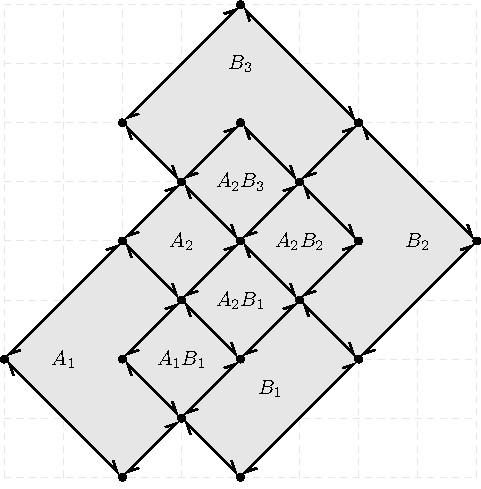
\includegraphics[scale=0.75]{figures/04/DCELUnion}};
        \node[node1,label={$A \cap B$}]           at (7,0)  {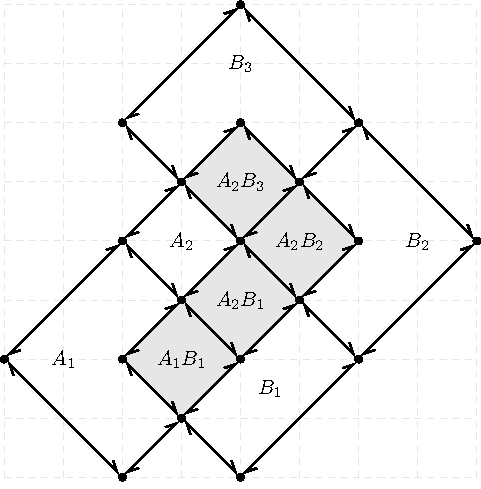
\includegraphics[scale=0.75]{figures/04/DCELIntersection}};
        \node[node1,label={$A \setminus B$}]      at (14,0) {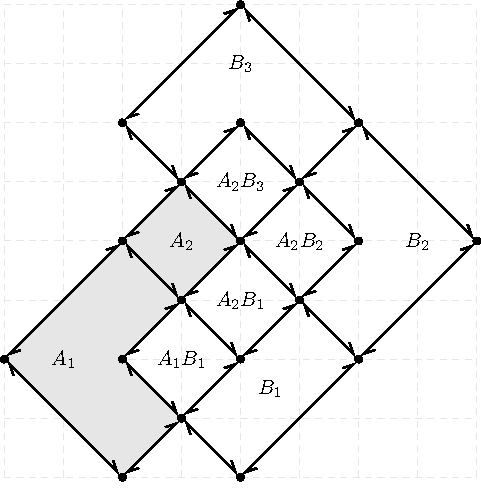
\includegraphics[scale=0.75]{figures/04/DCELDiffA}};
        \node[node1,label={$B \setminus A$}]      at (21,0) {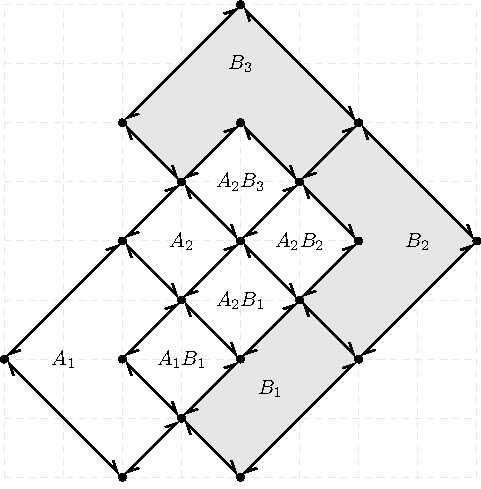
\includegraphics[scale=0.75]{figures/04/DCELDiffB}};
        \node[node1,label={$A \bigtriangleup B$}] at (28,0) {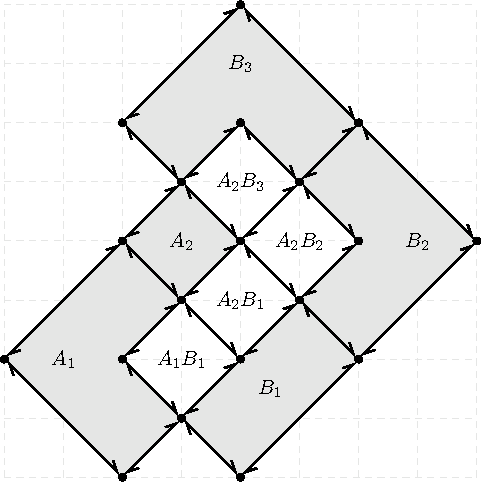
\includegraphics[scale=0.75]{figures/04/DCELDiff}};
    \end{tikzpicture}
}
    \caption{Examples of overlay operators supported by DCEL.}\label{fig:overlay_operations}
    \Description[Results of the overlay operations]{This figure shows the results of the overlay operations supported by the scalable DCEL.}
\end{figure*}

The current challenge is the construction of a distributed and scalable DCEL structure that allows the querying of overlay operations, such as intersection and difference, over a large set of polygons.  The main idea of the solution is to partition the edges from each of the polygons using a spatial data structure (for instance, a quadtree).  Edges contained at each section of the partitioning will be the input of a local DCEL which will store the information of the vertices, half-edges and faces for their edges clipped to the boundary of its spatial partition.  Each local DCEL can be seen as an individual structure which can be queried and the solution will be later merged with the other local DCELs in their neighbourhood to complete the final answer. 

\section{Scalable Overlay Construction} \label{sec:methods}

\subsection{Partition strategy} \label{sec:strategy}
The main idea of this strategy is to split the study area into a number of cells which could be processed independently in a local basis. We can take the case of the overlay operators over layers of polygons as an example to explains the details. In the parallel approach, the DCEL for each layer will be built independently at each cell following the sequential algorithm and then both will be merged to generate a structure where the operator can be applied.  

Our goal is to create DCELs for each layer in parallel to be able to solve large datasets the sequential alternatives are unable.  The proposal can be summarized in the following steps: (i) Partition the input polygons and build local DCEL representations of them at each partition; (ii) Merge the local DCELs for each layer together locally scaling the processing cost; (iii) Overlay operator can be run over the local merged DCELs to finally be collected back to mix and generate the final answer.  

The proposed partition schema is illustrated in figure \ref{fig:overlay_parted}.  First, we will use a sample of edges from both layers to create a set of cells which will spatially partition the space into disjoint areas.  In the example, a simple grid is used but any spatial index can be applied (in our experiments we use quadtrees for better balance and data distribution).  We will use those cells to clip the input polygons to generate new ones that will lie inside of the boundaries of the cell ensuring that all the needed edges for computation are available at each partition.  Although it will increase the number of edges and the size of the data, we expect that that the gain during parallel processing will make the addition worthwhile.

\begin{figure*}[!ht]
    \centering
    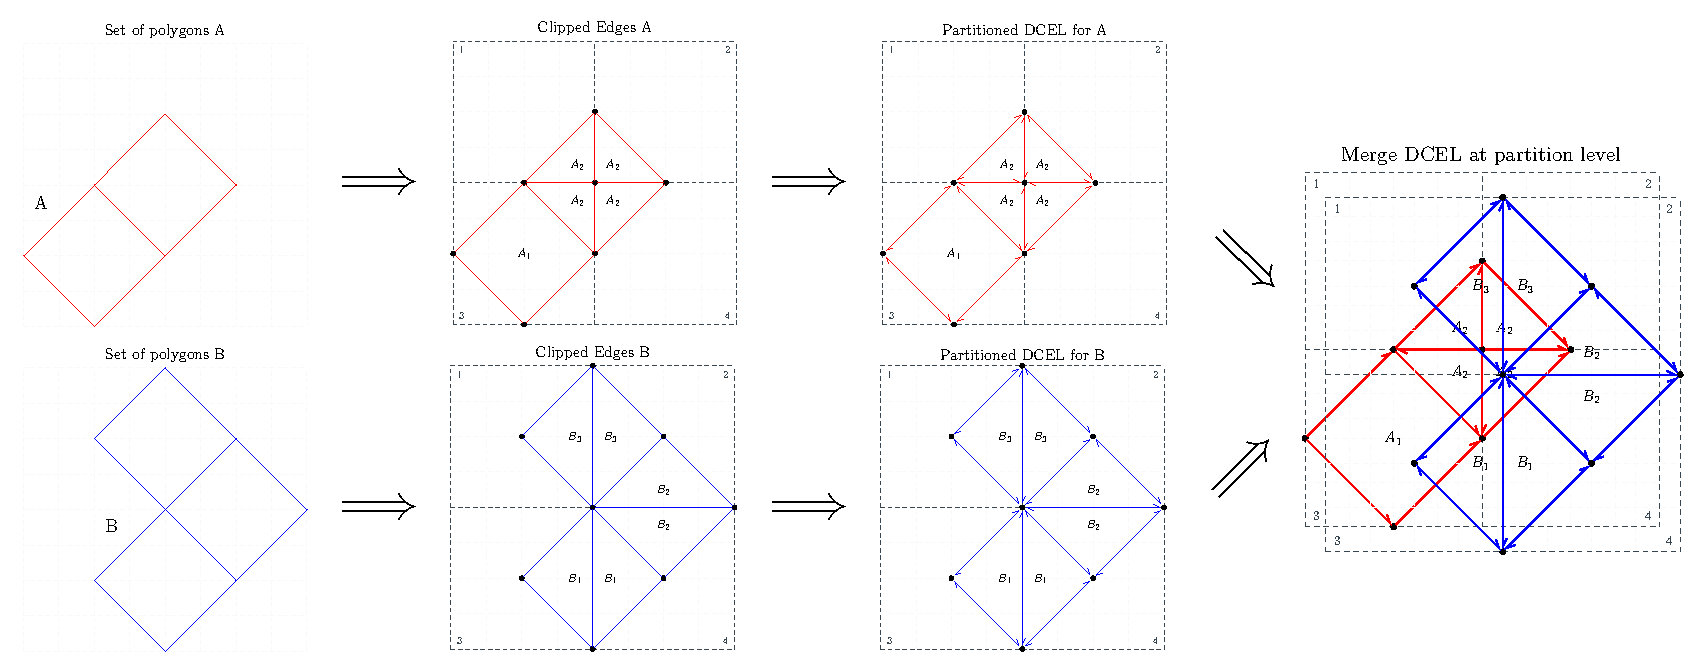
\includegraphics[width=\textwidth]{figures/01-OverlayParted}
    \caption{Partition scheme.}\label{fig:overlay_parted}
    \Description[Partition schema]{This figure illustrates the partition schema used to distribute the data.}
\end{figure*}

Now each cell have the enough data to build a DCEL representation of the polygons for each layer.  Data for each cell will be marked appropriately and submitted to different nodes to be processed in parallel.  Note that the same partition schema (set and shape of cells) is used in both layers.  That is important due to it allows one-to-one matching between corresponding partitions in both layers.

During the local DCEL construction for individual layers, it is straightforward the connection between the edges inside of each polygon.  From the inputs, it can easily be identified the position of each edge relate to its next and previous edges and to which face (polygon) the edge belongs.  It helps significantly the setting of the pointers required by each half-edge.   Using this, each edge is converted to a half-edge and their pointers are update accordingly.  However, a query to identify the twin pointer of each half-edge is still needed given that the input polygons do not provide which polygons are in its neighborhood. The matching is done through a self-join query among the current half-edges to pair those which share the same vertices in opposite directions.

However, when we pair the partitions from the both layers, we got two local DCELs (each representing the polygons for each layer) and the processing we need now is a merge between both of them.  It requires: (i) Identify the intersection points between the half-edges of each local DCEL and add them as new vertices; (ii) Split those half-edges involve in an intersection with a recently added vertex (prune duplicates if needed); (iii) Traverse the list of vertices and update their incident half-edge list; (iv) Update the pointers for next and previous half-edges in those affected by the splits; (v) Update the list of faces and their corresponding labels.

Figure \ref{fig:part2} depicts an overview of the process taking as example the polygons and edges of partition 2 of figure \ref{fig:overlay_parted}.  Similarly, figure \ref{fig:merged_dcel} shows the full result of the merged DCEL once all the partitions have processed their corresponding edges. Note that red half-edges have been introduced artificially by the partition strategy but they are marked accordingly to be used and removed after the collect back process when we need to unify the results after the application of the overlay operators.

\begin{figure}
    \centering
    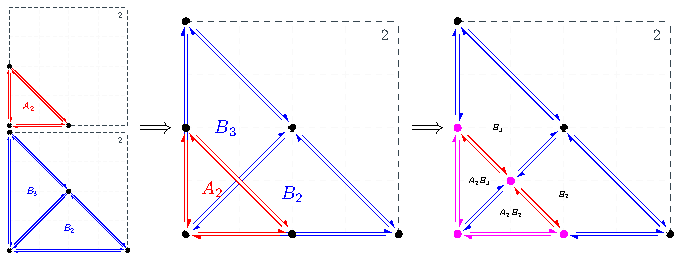
\includegraphics[width=0.9\linewidth]{figures/02-Part2}
    \caption{Overlay of local DCEL for partition 2.}\label{fig:part2}
    \Description[Overlay of local DCELs for a particular partition]{This figure shows how the local DCELs works in a particular example.}
\end{figure}

\begin{figure}[!ht]
    \centering
    \tikzset{    
    barbarrow/.style={ % style that just defines the arrow tip
        %>={Straight Barb[left,length=5pt,width=5pt]},
        >={Triangle[left,length=5pt,width=5pt]},
        double,
        semithick,
        <->
    },
    whites/.style={
        thick, 
        color=white
    }
}
\definecolor{light-gray}{gray}{0.9}
\scalebox{0.75}{
\begin{tikzpicture}
    \tikzstyle{node1}=[draw,scale=0.4,shape=circle,color=black,fill=black]
    \tikzstyle{node2}=[draw,scale=0.4,shape=circle,color=red,fill=red]    
    \draw[color=light-gray, style=dashed] (0,0) grid (8,8);
    \draw[color=red, style=dashed, step=4] (0,0) grid (8,8);
    \node[node1] (A) at (0,2) {};    \node[node1] (C) at (2,0) {};
    \node[node1] (D) at (2,2) {};    \node[node1] (E) at (2,4) {};
    \node[node1] (F) at (2,6) {};    \node[node1] (G) at (3,1) {};
    \node[node1] (H) at (3,3) {};    \node[node1] (I) at (3,5) {};
    \node[node1] (J) at (4,0) {};    \node[node1] (K) at (4,2) {};
    \node[node1] (L) at (4,4) {};    \node[node1] (M) at (4,6) {};
    \node[node1] (N) at (4,8) {};    \node[node1] (O) at (5,3) {};
    \node[node1] (P) at (5,5) {};    \node[node1] (Q) at (6,2) {};
    \node[node1] (R) at (6,4) {};    \node[node1] (S) at (6,6) {};
    \node[node1] (T) at (8,4) {};

    \node at (1,2)      {$A_1$};
    \node at (6.5,4.6)  {$B_2$};
    \node at (6.5,3.4)  {$B_2$};
    \node at (3.4,6.5)  {$B_3$};
    \node at (4.6,6.5)  {$B_3$};
    \node at (4.6,1.5)  {$B_1$};
    \node at (3.6,1)    {$B_1$};
    \node at (3,4.4)    {$A_2$};
    \node at (3,3.6)    {$A_2$};
    \node at (3,2)              {$A_1B_1$};
    \node[scale=0.6] at (3.6,3) {$A_2B_1$};
    \node[scale=0.6] at (4.4,3) {$A_2B_1$};
    \node[scale=0.6] at (5,4.4) {$A_2B_2$};
    \node[scale=0.6] at (5,3.6) {$A_2B_2$};
    \node[scale=0.6] at (3.6,5) {$A_2B_3$};
    \node[scale=0.6] at (4.4,5) {$A_2B_3$};
    
    \draw[barbarrow] (A) -- (C);\draw[barbarrow] (A) -- (E);
    \draw[barbarrow] (C) -- (G);\draw[barbarrow] (D) -- (G);
    \draw[barbarrow] (D) -- (H);\draw[barbarrow] (E) -- (H);
    \draw[barbarrow] (E) -- (I);\draw[barbarrow] (F) -- (I);
    \draw[barbarrow] (F) -- (N);\draw[barbarrow] (G) -- (J);
    \draw[barbarrow] (H) -- (L);\draw[barbarrow] (I) -- (L);
    \draw[barbarrow] (I) -- (M);\draw[barbarrow] (J) -- (Q);
    \draw[barbarrow] (G) -- (K);\draw[barbarrow] (H) -- (K);
    \draw[barbarrow] (K) -- (O);\draw[barbarrow] (L) -- (O);
    \draw[barbarrow] (L) -- (P);\draw[barbarrow] (M) -- (P);
    \draw[barbarrow] (N) -- (S);\draw[barbarrow] (O) -- (Q);
    \draw[barbarrow] (O) -- (R);\draw[barbarrow] (P) -- (R);
    \draw[barbarrow] (P) -- (S);\draw[barbarrow] (Q) -- (T);
    \draw[barbarrow] (S) -- (T);
    
    \draw[whites] (A) -- (C);\draw[whites] (A) -- (E);
    \draw[whites] (C) -- (G);\draw[whites] (D) -- (G);
    \draw[whites] (D) -- (H);\draw[whites] (E) -- (H);
    \draw[whites] (E) -- (I);\draw[whites] (F) -- (I);
    \draw[whites] (F) -- (N);\draw[whites] (G) -- (J);
    \draw[whites] (H) -- (L);\draw[whites] (I) -- (L);
    \draw[whites] (I) -- (M);\draw[whites] (J) -- (Q);
    \draw[whites] (G) -- (K);\draw[whites] (H) -- (K);
    \draw[whites] (K) -- (O);\draw[whites] (L) -- (O);
    \draw[whites] (L) -- (P);\draw[whites] (M) -- (P);
    \draw[whites] (N) -- (S);\draw[whites] (O) -- (Q);
    \draw[whites] (O) -- (R);\draw[whites] (P) -- (R);
    \draw[whites] (P) -- (S);\draw[whites] (Q) -- (T);
    \draw[whites] (S) -- (T);
    
    \draw[barbarrow, color=red] (R) -- (T);\draw[whites] (R) -- (T);
    \draw[barbarrow, color=red] (M) -- (N);\draw[whites] (M) -- (N);
    \draw[barbarrow, color=red] (K) -- (J);\draw[whites] (K) -- (J);
    \draw[barbarrow, color=red] (L) -- (E);\draw[whites] (L) -- (E);
    \draw[barbarrow, color=red] (L) -- (R);\draw[whites] (L) -- (R);
    \draw[barbarrow, color=red] (L) -- (M);\draw[whites] (L) -- (M);
    \draw[barbarrow, color=red] (L) -- (K);\draw[whites] (L) -- (K);
\end{tikzpicture}
}    
    \caption{Result of the merged DCEL.}\label{fig:merged_dcel}
    \Description[Result of the merged DCEL]{This figure shows what would be the results of the merge DCEL procedure.}
\end{figure}

At this point, we have access to a distributed spatial data structure which collects the individual DCEL representations (and its topological and geometric information) of the full study area at local basis.  It is easy to see that we can run overlay operators in parallel over the local DCELs and then just collect and merge the results to unify a final answer.  For example, figure \ref{fig:overlay_parted2} illustrates the process to query for the intersection results over the input polygons described in figure \ref{fig:overlay_parted}.  

\begin{figure}[!ht]
    \centering
    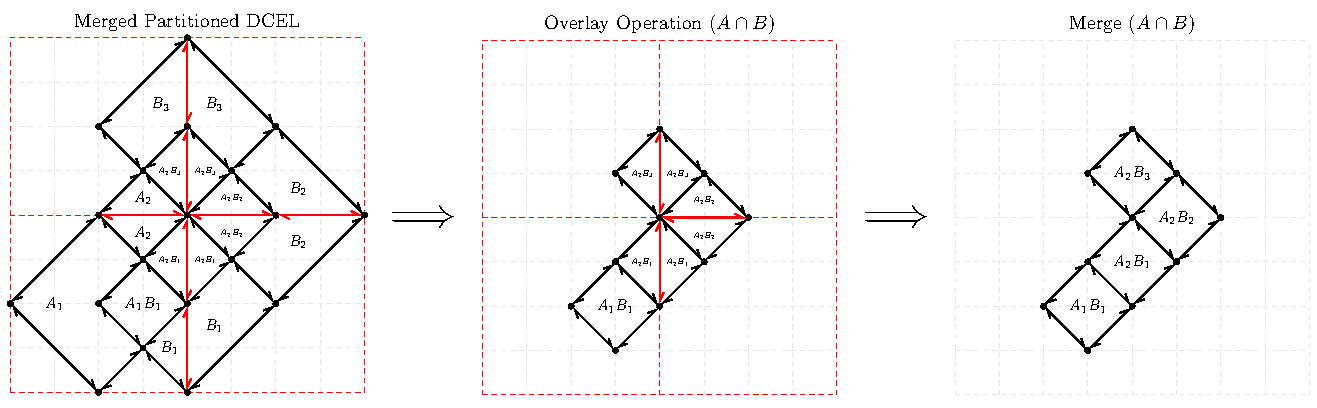
\includegraphics[width=\linewidth]{figures/03-OverlayParted2}
    \caption{Example of an overlay operation querying the distributed DCEL.} \label{fig:overlay_parted2}
    \Description[An example of an overlay operation]{This figure shows an example of an overlay operation querying the distributed DCEL.}
\end{figure}

The results of the overlay operators supported by the scalable DCEL are the same shown in figure \ref{fig:overlay_operations}.  To obtain the results the faces are filtered locally according to the characteristics of their label.  For intersection ($A \cap B$), it filters just faces where its label contains both letters (A and B); for symmetric difference ($A \bigtriangleup B$), it filters faces where its labels contains just one of the letters (A or B).  For the case of difference between the layers ($A \setminus B$ or $B \setminus A$), it filters faces and labels according to the requested letter (either A or B). In the case of union ($A \cup B$), all the faces are retrieved. 

\subsection{Parallel DCEL Computation}

During the partition process, the edges of each polygon are attached with pointers to their next and previous edge according to their order in the polygon's vertices.  As explained before, a spatial index is used to assign each edge to a particular cell.  Each edge is queried in the spatial data structure and it is labeled with the cell where it is contained.  If a edge covers multiples cell it is replicated in each one but clipped to the corresponding cell boundary.  In addition, edges representing the boundary of the cell are added to complement the edges enclosed in each cell.  Those artificial edges are marked accordingly to be removed during the merge stage.

The edges of the cell added at this stage are useful to complete the local DCEL.  It will allow that the resulting DCEL will enclose the full area of the cell and the local DCEL at each cell matches with the local DCEL of the other layer during the merge process.  The half-edges which intersect the boundary of the cell will be connected to the edges of the boundary to form closed faces to obtain the global DCEL.

As the edges have been partitioned accordingly to the spatial index, each cell will contain all the data they need to process and compute a DCEL locally in a parallel fashion. In each case, after the DCEL is built those half-edges and faces that are not involved with the edges introduced by the boundary of the cell could be reported directly and they do not need additional analysis.  It is, most of the edges in the middle of the cell which do not have contact to the boundary are ready for the merging stage and they do not need additional workload.  It is expected that most of the work can be done inside the cell taking advantage of parallelism.

On the other hand, those edges which are connected to the border of the cell must be further processed.  Those edges can extend to adjacent cells in their neighborhood and build more complex faces.  During the merge stage, those half-edges are collected and compared to see if other half-edges in the neighbourhood matches and must be extended.  In general, the open half-edges are evaluated in a master node where it searches for additional ones with the same label and concatenate them accordingly to form closed faces.  In section ~\ref{sec:optimizing} a couple of techniques to optimize the merging process of this kind of half-edges are proposed.  

\subsection{Cell inside polygon problem} \label{sec:anomalies}
The main goal of the proposal is to be able to divide the problem into smaller partitions for efficient processing.  Each partition collects the needed data and it is able to build its local DCEL without the need of query other partitions.  However, under this partition strategy, a new problem arises.  It happens when the partition schema (i.e. a quadtree) deliver a cell where no edges for any of the input layers are located.  The problem is even more complicated when just a hole in located inside a cell (figure \ref{fig:emptycells}).  The problem is that the empty cell (or the empty portion in the case of holes) has no access to which polygon it belongs making its corresponding labeling impossible.  

%\begin{figure}[!ht]
%    \centering
%    \includegraphics[page=2, width=0.25\textwidth]{figures/cellinpolygon/emptycells.pdf}
%    \caption{Example of empty cell and empty cell with holes cases.}\label{fig:emptycells}
 %   \Description[Examples of empty cells]{This figure shows some examples of of empty cell and empty cell with holes cases.}
%\end{figure}

To solve the problem, an algorithm is proposed to find the closest cell with the valid information about the polygon they are contained.  It is based on the branch information of the cell inside of the spatial index structure used during partition, also know as lineage.  For the sack of explanation, we will assume we use a quadtree, but the proposal could be easily adapted to other index structures.

After the partitioning strategy, a set of the cells is available with the following information: an unique cell identifier; a lineage as a string which provides the position and depth of the cell into the spatial index; and an envelope which is a polygon representation (a rectangle) of the boundaries of the cell.

The key of the proposal is to identify the centroid of the parent cell from the current empty cell in question.  That point will allow us to retrieve the neighbour cells which can easily be queried if they have edges to extract the needed polygon information.  If all of them are still empty, we proceed to choose that one with the deepest level and recursively repeat the process.  Eventually, a non-empty cell will emerge and all the involved empty cells can be updated.  Figure \ref{fig:emptycellexample} shows a three-iteration run of the algorithm.

\begin{figure*}
    \centering
    \includegraphics[page=2, width=0.24\linewidth]{figures/cellinpolygon/emptycells}
    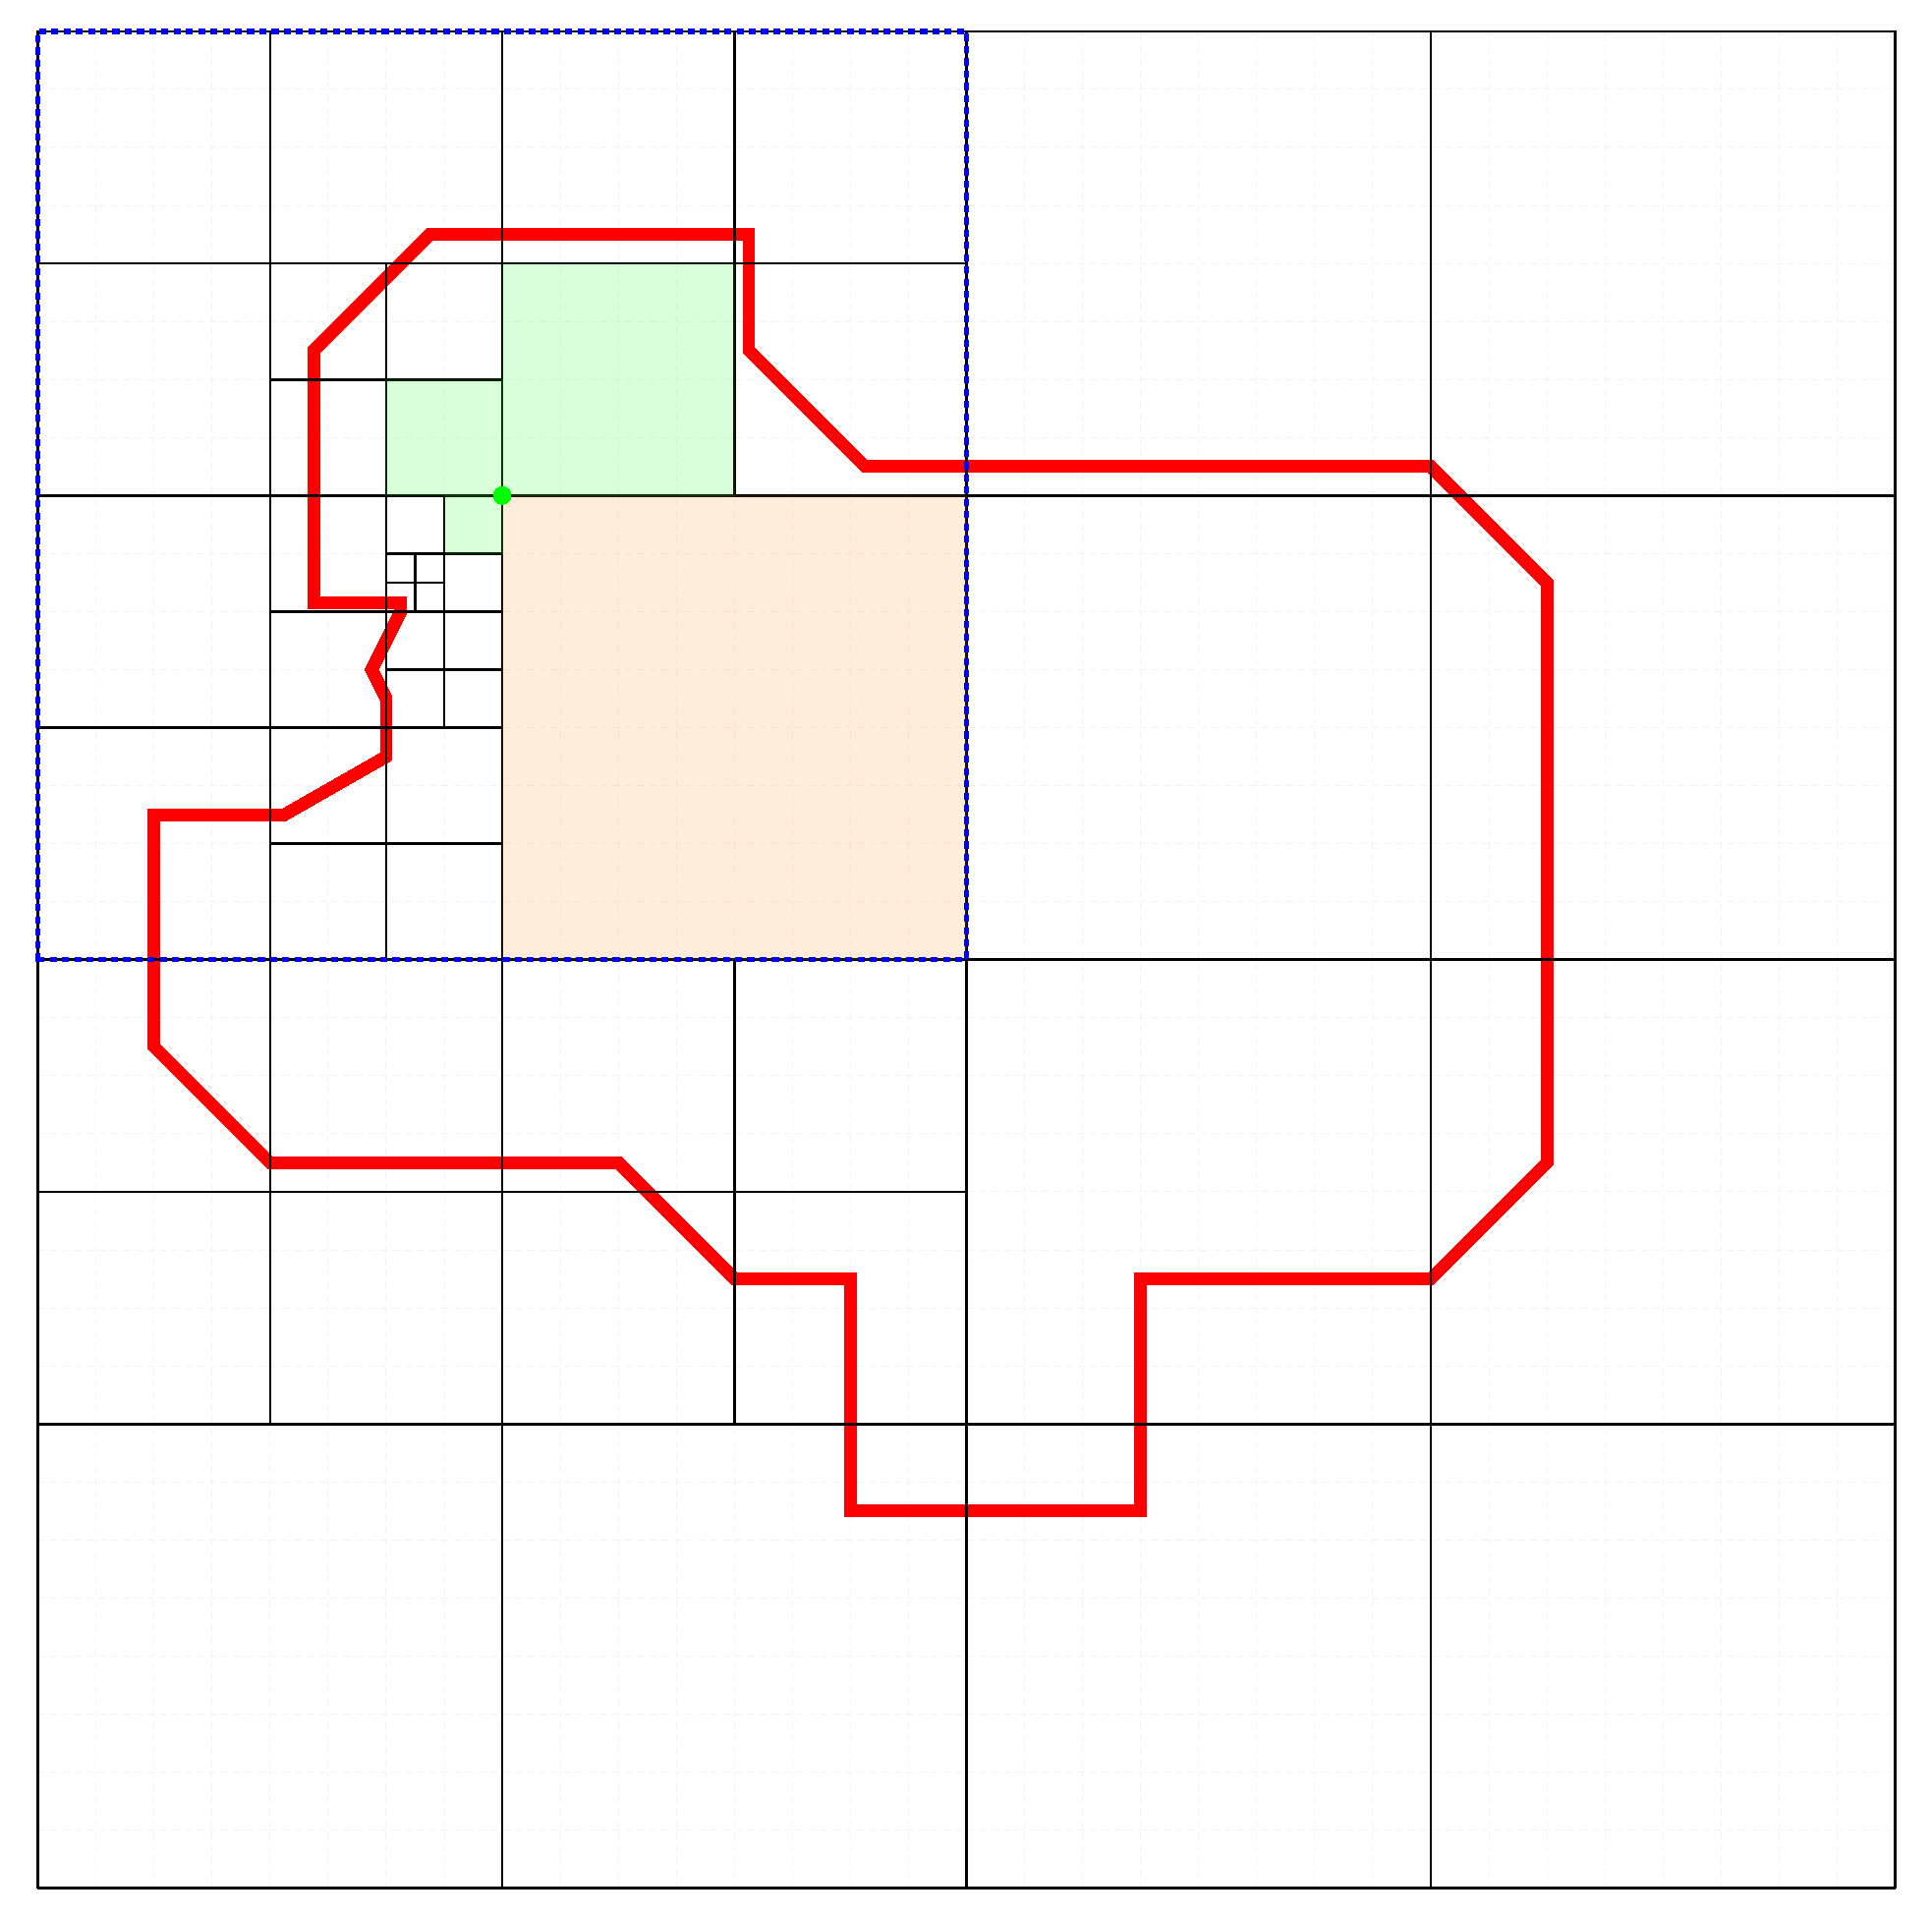
\includegraphics[page=1, width=0.24\linewidth]{figures/cellinpolygon/example}
    \includegraphics[page=2, width=0.24\linewidth]{figures/cellinpolygon/example}
    \includegraphics[page=3, width=0.24\linewidth]{figures/cellinpolygon/example}
    \caption{Three iterations of the proposed algorithm to find the next cell with valid edges from a empty cell.} \label{fig:emptycellexample}
    \Description[Iteration of the proposed algorithm]{This figure shows three iterations of the proposed algorithm to find the next cell with valid edges from a empty cell.}
\end{figure*}

The details and pseudo code of the algorithm can be seen at Algorithms \ref{alg:one} and \ref{alg:two}.  They explain the steps to obtain a near quadtree cell which guarantee the presence of edges and how select the set of three cells around of a given corner respectively.  The latter is used to choose a possible path if the current cell is empty and it needs to identify at which polygon it belongs.  The former (using the latter) ensures the finding of a cell with the polygons' edges needed to determine the enclosing polygon.

\begin{algorithm}\caption{\textsc{getNextCellWithEdges} algorithm}\label{alg:one}
    \begin{algorithmic}[1]
    \Require a quadtree with cell envelopes $\mathcal Q$ and map of cells and their edge count $\mathcal M$.
    \Function{ getNextCellWithEdges }{ $\mathcal Q$, $\mathcal M$ }
        \State $\mathcal C \gets $ list of empty cells in $\mathcal M$
        \ForEach{ $emptyCell$ in $\mathcal C $ }
            \State initialize $cellList$ with $emptyCell$ 
            \State $nextCellWithEdges \gets null$
            \State $referenceCorner \gets null$
            \State $done \gets false$
            \While{ not $done$ } 
                \State $c \gets $ last cell in $cellList$ 
                \State $cells, corner \gets \textsc{getCellsAtCorner}(\mathcal Q, c)$ \Comment{ return 3 cells and the reference corner }
                \ForEach{$cell$ in $cells$}
                    \State $nedges \gets$ get edge count of $cell$ in $\mathcal M$ 
                    \If{ $nedges > 0$ }
                        \State $nextCellWithEdges \gets cell$
                        \State $referenceCorner \gets corner$
                        \State $done \gets true$
                    \Else
                        \State add $cell$ to $cellList$
                    \EndIf
                \EndFor
            \EndWhile
            \ForEach{ $cell$ in $cellList$ }
                \State \textbf{output}($cell$, \\
                \hspace{2.5cm} $nextCellWithEdges$, $referenceCorner$)
                \State remove $cell$ from $\mathcal C$
            \EndFor
        \EndFor
    \EndFunction
    \end{algorithmic}
\end{algorithm}

\begin{algorithm} \caption{\textsc{getCellsAtCorner} algorithm}\label{alg:two}
    \begin{algorithmic}[1]
    \Require a quadtree with cell envelopes $\mathcal Q$ and a cell $c$.
    \Function{ getCellsInCorner }{ $\mathcal Q$, $c$ }
        \State $region \gets $ last character in $c.lineage$
        \Switch{ $region$ }
            \Case{ `0' }
                \State $corner \gets$ left bottom corner of $c.envelope$
            \EndCase
            \Case{ `1' }
                \State $corner \gets$ right bottom corner of $c.envelope$
            \EndCase
            \Case{ `2' }
                \State $corner \gets$ left upper corner of $c.envelope$
            \EndCase
            \Case{ `3' }
                \State $corner \gets$ right upper corner of $c.envelope$
            \EndCase
        \EndSwitch
        \State $cells \gets$ cells which intersect $corner$ in $\mathcal Q$
        \State $cells \gets cells - c$ \Comment{ Remove the current cell from the intersected cells }
        \State $cells \gets$ sort $cells$ on basis of their depth \Comment{ using $cell.lineage$ }
        \State \Return{ ($cells$, $corner$) }
    \EndFunction
    \end{algorithmic}
\end{algorithm}

We based of proposal in the following lemma and used it to proved our point with the subsequent proof.

\begin{lemma}
Four cells at the same level can not be empty.  At least one of them must have edges in order to force the split.
\end{lemma}

\begin{proof}
The $\textsc{getCellsInCorner}$ function will query the interior corner of a cell according to its position, that is the centroid of its cell parent.  The only cells which can intersect that point are cells at the same level of the current cell or their children.  If the 3 cells returned by $\textsc{getCellsInCorner}$ are empty, at least one of them must have a deeper level that the current cell.  Following that cell guarantees that the search space will be shrank at each iteration.  Eventually, the algorithm will reach the maximum level of the quadtree where all the involved cells will have the same level and, therefore, at least one of them must have edges.
\end{proof}

\subsection{Merging stage for computing final results} \label{sec:merge}
Once the distributed DCEL is ready for analysis, we have to take care on how it should be queried in order to take advantage of such distribution.  Section \ref{sec:strategy} shows the initial strategy to partition the study area and how each partition holds a section of the DCEL clipped to the cell boundary of that partition.  It is straightforward that we could query locally each of the sections but, once it is done, we should unify the results among contiguous partitions.

Faces in the interior of a partition (those which do not touch the boundary) are safe to be reported.  However, for those faces which share a half-edge with the boundary, there is a high chance that another section of that face is present in a contiguous cell and has to be checked.  

We execute a merging stage on the set of faces which touch the boundaries of each partition.  It performs a reduce operation pairing faces with the same label and dissolving their geometries.  For example, in figure \ref{fig:overlay_parted2}, it can be seen how faces in different partitions but with the same label are merged into final results by removing their common half-edges. 

\section{Overlay evaluation optimizations}\label{sec:alternative_methods}
\subsection{Optimizing for polygons expanding partitions.}\label{sec:optimizing}
To evaluate the best alternatives during the reduce/merge stage, three different approaches were evaluated to glue together segments of faces which could be located in different cells.  Those closed segments which form auto-contained faces inside of each partition are immediately reported and there is no need for additional processing.  However, those segments which touch the border of the cell in their partition must be post-processed to evaluate if they could be extended with segments in their proximity.

The first naive approach was to collect those segments in a master/root node which sequentially will combine them with the same labels and concatenate them accordingly in order to create the final and consolidated answer.  It is a straightforward method but could be really costly if the number of partitions and the subsequent number of segments touching the borders are relatively large.

As an alternative, it is proposed to do an intermediate step with a parameter introduced by the user were a level in the quadtree structure is given.  Following this parameter, the segments in partitions below the given level are collect them in intermediate nodes of the quadtree were can be evaluated partially.  The goal of this step is that part of the work can be distributed in a larger number of nodes as a previous step before to be sent to the master/root node for final evaluation.  It is expected that most of the work can be done in the intermediate step.  However, those partitions located above of the level still have to be evaluated in an individual node.

It is clear that it will create an optimization issue: if we choose a level low in the structure it can be evaluated in a larger number of intermediate nodes (taking advantage of parallelism) but, at the same time, a large number of partitions will be located above of that threshold and they will be evaluated by an unique node which can dominate the execution time.  On the other hand, if a level is selected high in the quadtree, just a few number of partitions will have to be evaluated in that unique node, but the number of intermediate nodes will also be reduced and the execution time for their evaluation will increase.

Last method take a different approach.  It partitions the set of segments at each partition by their label itself.  It is, it will reorganize the segments using their labels as the key.  The resulting dataset will put together those segments which share the same label in the same partition and they will be evaluated in the same node.  In this case, the cost of the re-partitioning should be evaluated but it is expected than the number and size of the resulting partitions will take much more advantage of parallelism.

\subsection{Optimization in the presence of unbalanced layers.}\label{sec:unbalance}
Clearly the most time consuming operation is the overlay of the individual DCELs once they have been created for each layer.  Particularly, when the combination of half-edges from each layer is performing at each cell, the most critical task is finding the intersection points between the two sets of half-edges. In many cases the number of half-edges from each layer can be quiet unbalance, it is one of the cells has much more half-edges than the other.

In the traditional approach, a common sweep-line approach is performed scanning both sets of half-edges from left to right (scanning the x-axis) inside each cell and the corresponding intersections points are reported in order to continue with the creation of the merged DCEL (see Section \ref{sec:prelim}). This approach does not consider the fact that in some cells, one of the sets can be larger than the other and there is no need to scan all the half-edges in many cases.

An alternative approach is proposed for those cases.  It start detecting which set contains more half-edges and which has more probability to overlap the smaller one in the x-axis. Then, it performs a simple scan in the smaller to extract the wide of this dataset and returned in the form of intervals over the x-axis.  It has to be noted that a smaller dataset can extend in several intervals over the bigger dataset and it has been managed accordingly.  

With each interval, it is possible to locate the point in the x-axis where the sweep-line algorithm should start scanning from the bigger set and compared with the half-edges from de smaller one. On those cases where the bigger and smaller set differ considerably in size, it is possible to save time due to the fact that many sections of the bigger set do not required to be scanned nor compared with the smaller set.